\section{Μετατροπέας Υποβιβασμού}
Μοντελοποιήθηκε ένας μετατροπέας υποβιβασμού σύμφωνα με τις σχέσεις που αναφέρθηκαν στις υποενότητες \ref{Phase_1} και \ref{Phase_2} και στην συνέχεια κατασκευάστηκαν οι γραφικές ρεύματος πηνίου $I_L$, ρεύματος πυκνωτή $I_C$ και τάσης πυκνωτή $V_C$ για διαφορετικές τιμές του Duty Cycle και της αυτεπαγωγής L.

\subsection{Duty Cycle = 0.5  -  L = 0.001H}

\subsubsection{Ρεύμα πηνίου}
\begin{figure}[h!]
	\begin{subfigure}{\textwidth}
		\centering
		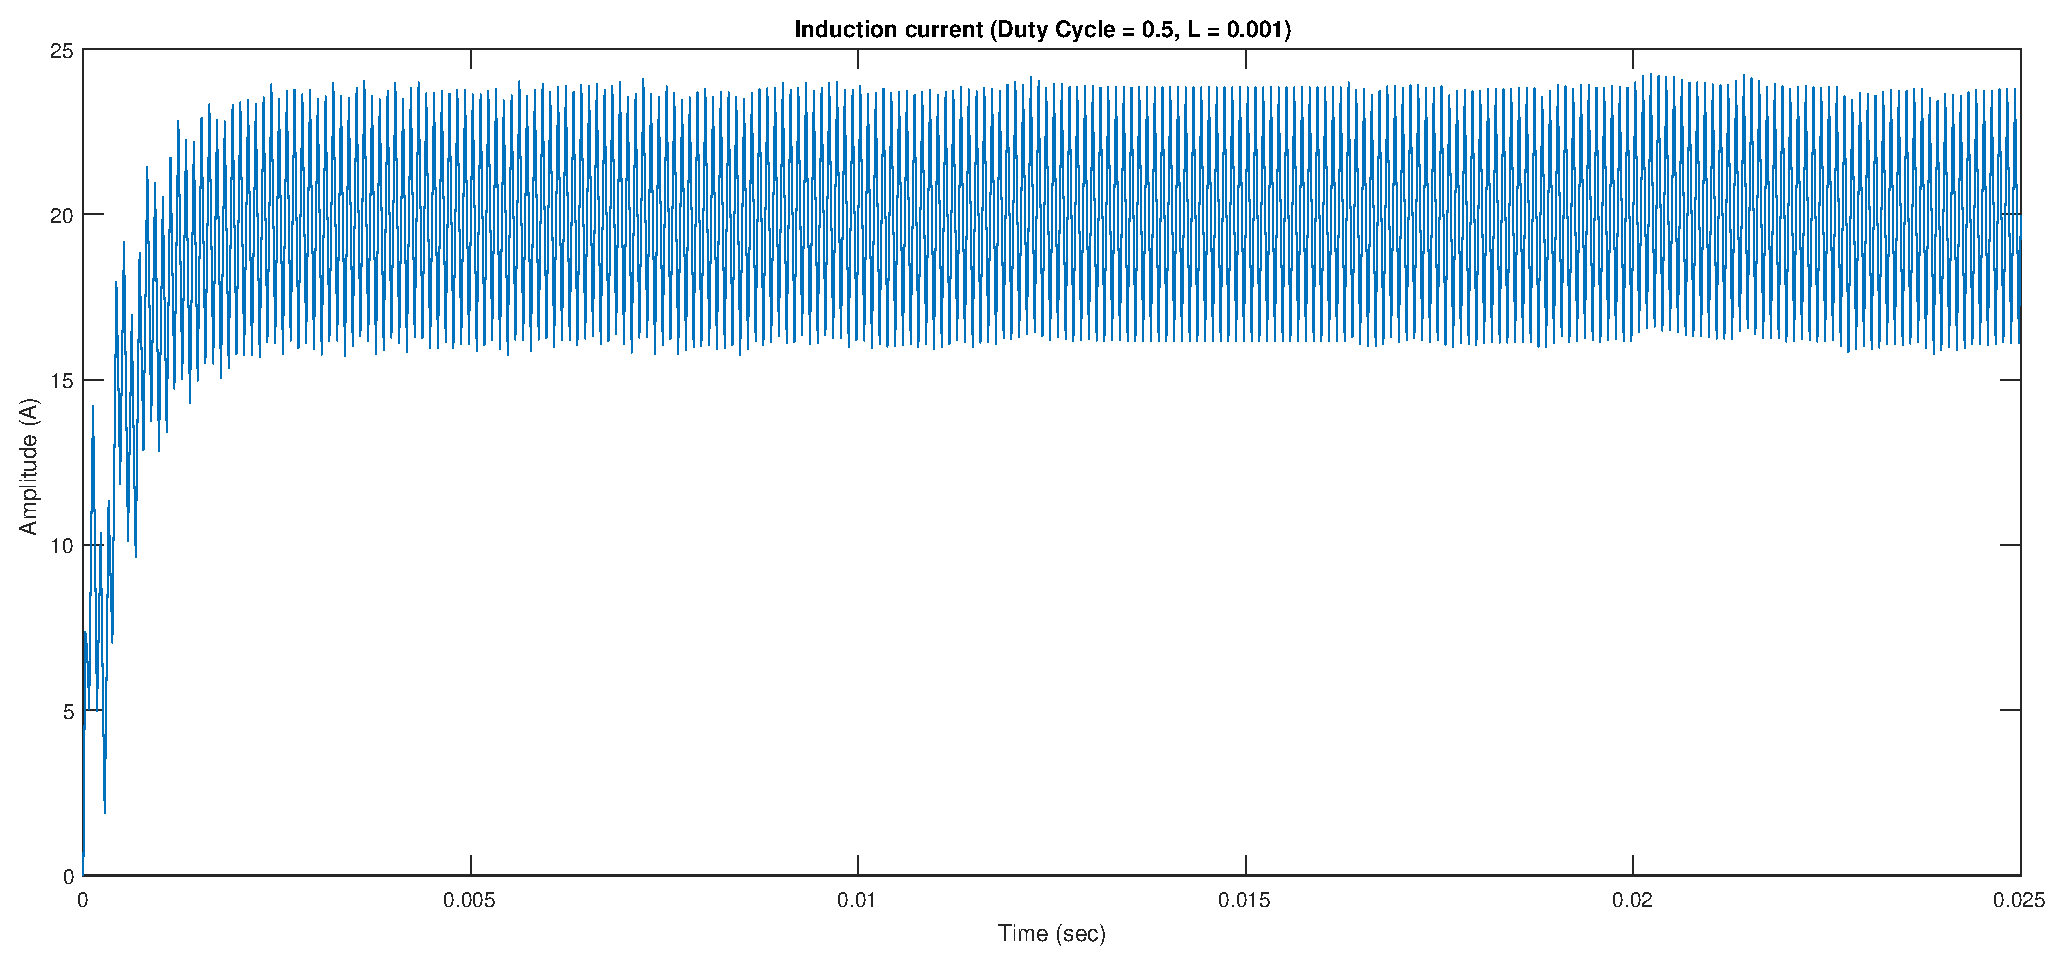
\includegraphics[width=0.7\textwidth]{Images/I_L_05_1}
	\end{subfigure}
	\\\\
	\begin{subfigure}{\textwidth}
		\centering
		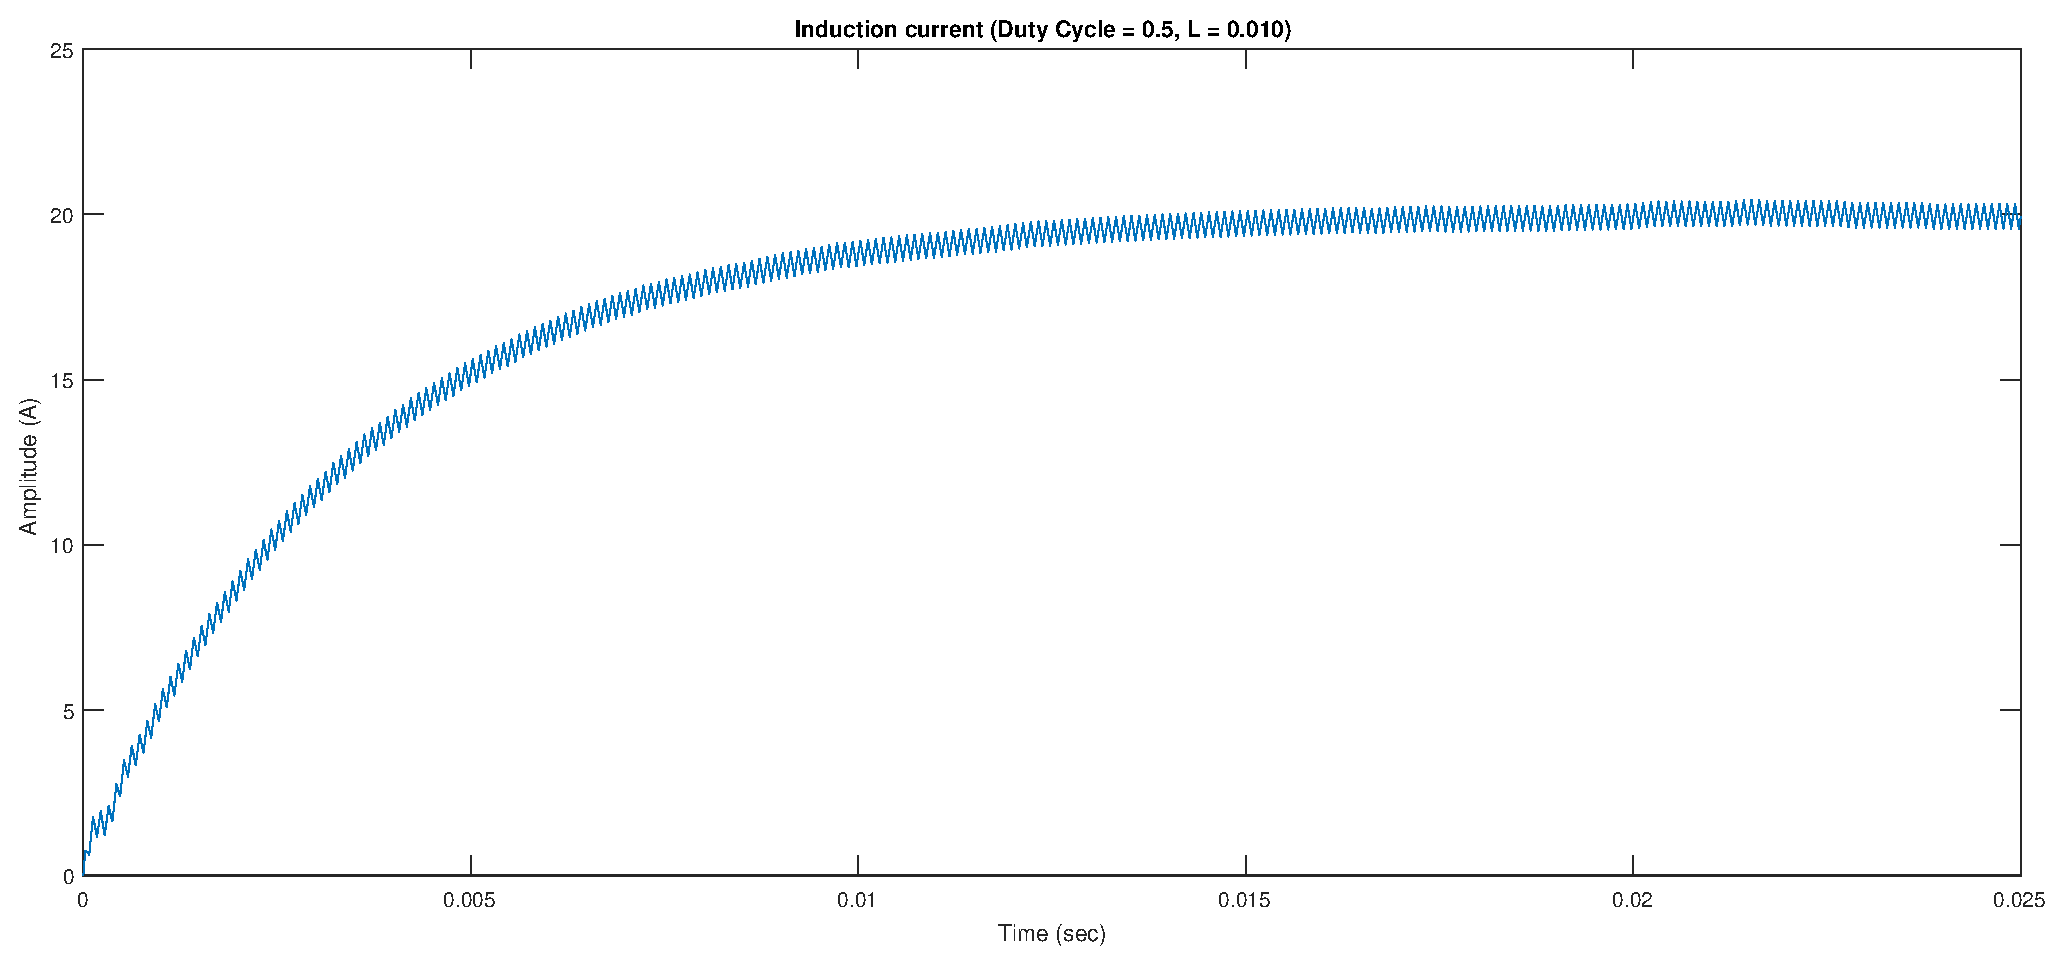
\includegraphics[width=0.7\textwidth]{Images/I_L_05_10}
	\end{subfigure}
	\\\\
	\begin{subfigure}{\textwidth}
		\centering
		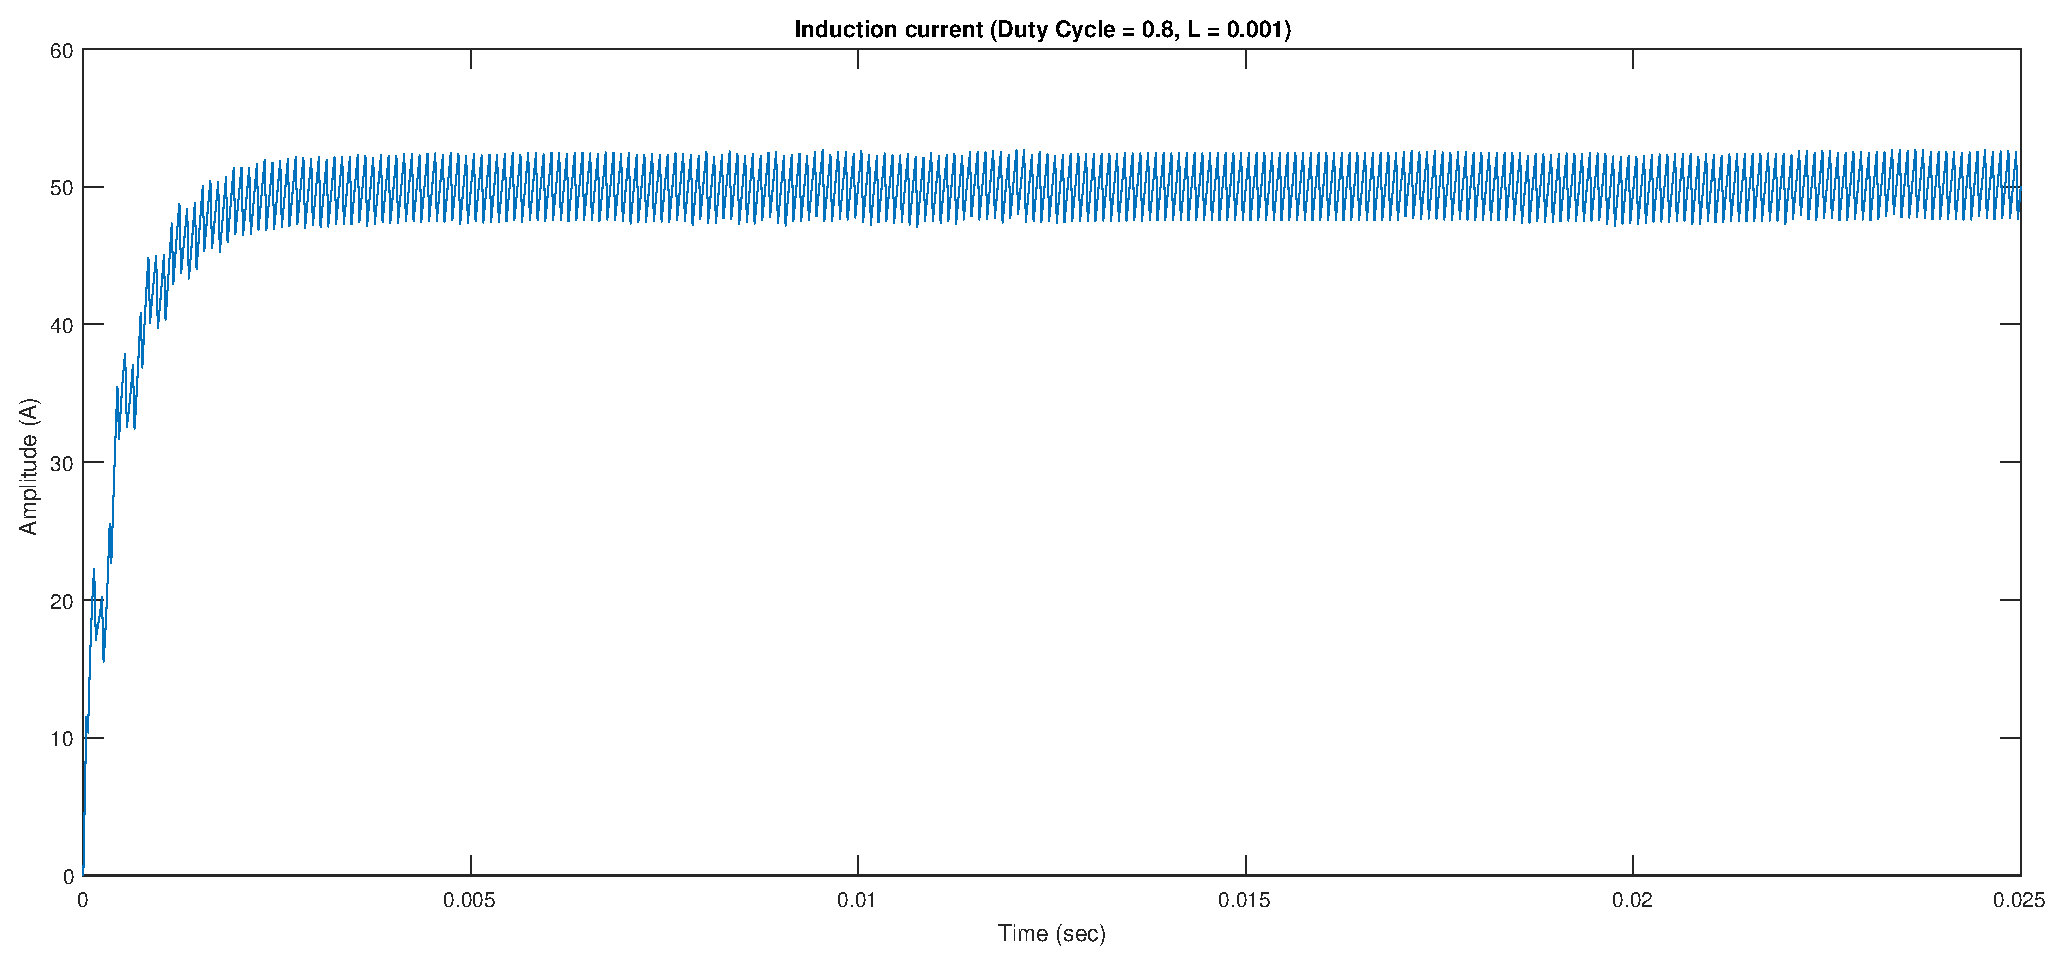
\includegraphics[width=0.7\textwidth]{Images/I_L_08_1}
	\end{subfigure}
\end{figure}
\noindent
Παρατηρώντας τις κυματομορφές του ρεύματος πηνίου είναι εμφανές πως ανάλογα με την περίπτωση, αλλάζει αρκετά η μορφή της γραφικής. Όσον αφορά το Duty Cycle, η αύξηση του επιφέρει αύξηση της μέση τιμής του ρεύματος όπως είναι εμφανές από την σύγκριση μεταξύ των πρώτων δύο γραφικών και της τρίτης, όπου η μέση τιμή διπλασιάζεται. Η συμπεριφορά αυτή ήταν αναμενόμενη σύμφωνα με τις σχέσεις (\ref{I_L_1}) και (\ref{I_L_2}). Να το πούμε λίγο καλύτερα αυτό.

\noindent\\
Αντίστοιχα, αυξάνοντας την αυτεπαγωγή L μειώνεται το πλάτος διακύμανσης του ρεύματος κάνοντάς το πιο σταθερό, ωστόσο αυξάνεται ο χρόνος σταθεροποίησης. Οι επιδράσεις αυτές οφείλονται στην φύση του πηνίου το οποίο τείνει να εξομαλύνει τις μεταβολές στο ρεύμα.
\noindent
Το ρεύμα του πηνίου στην δεδομένη περίπτωση παρουσιάζει μεγάλη διακύμανση και μέση τιμή γύρω στα 20Α.\\

\subsubsection{Ρεύμα πυκνωτή}
\begin{figure}[h!]
	\centering
	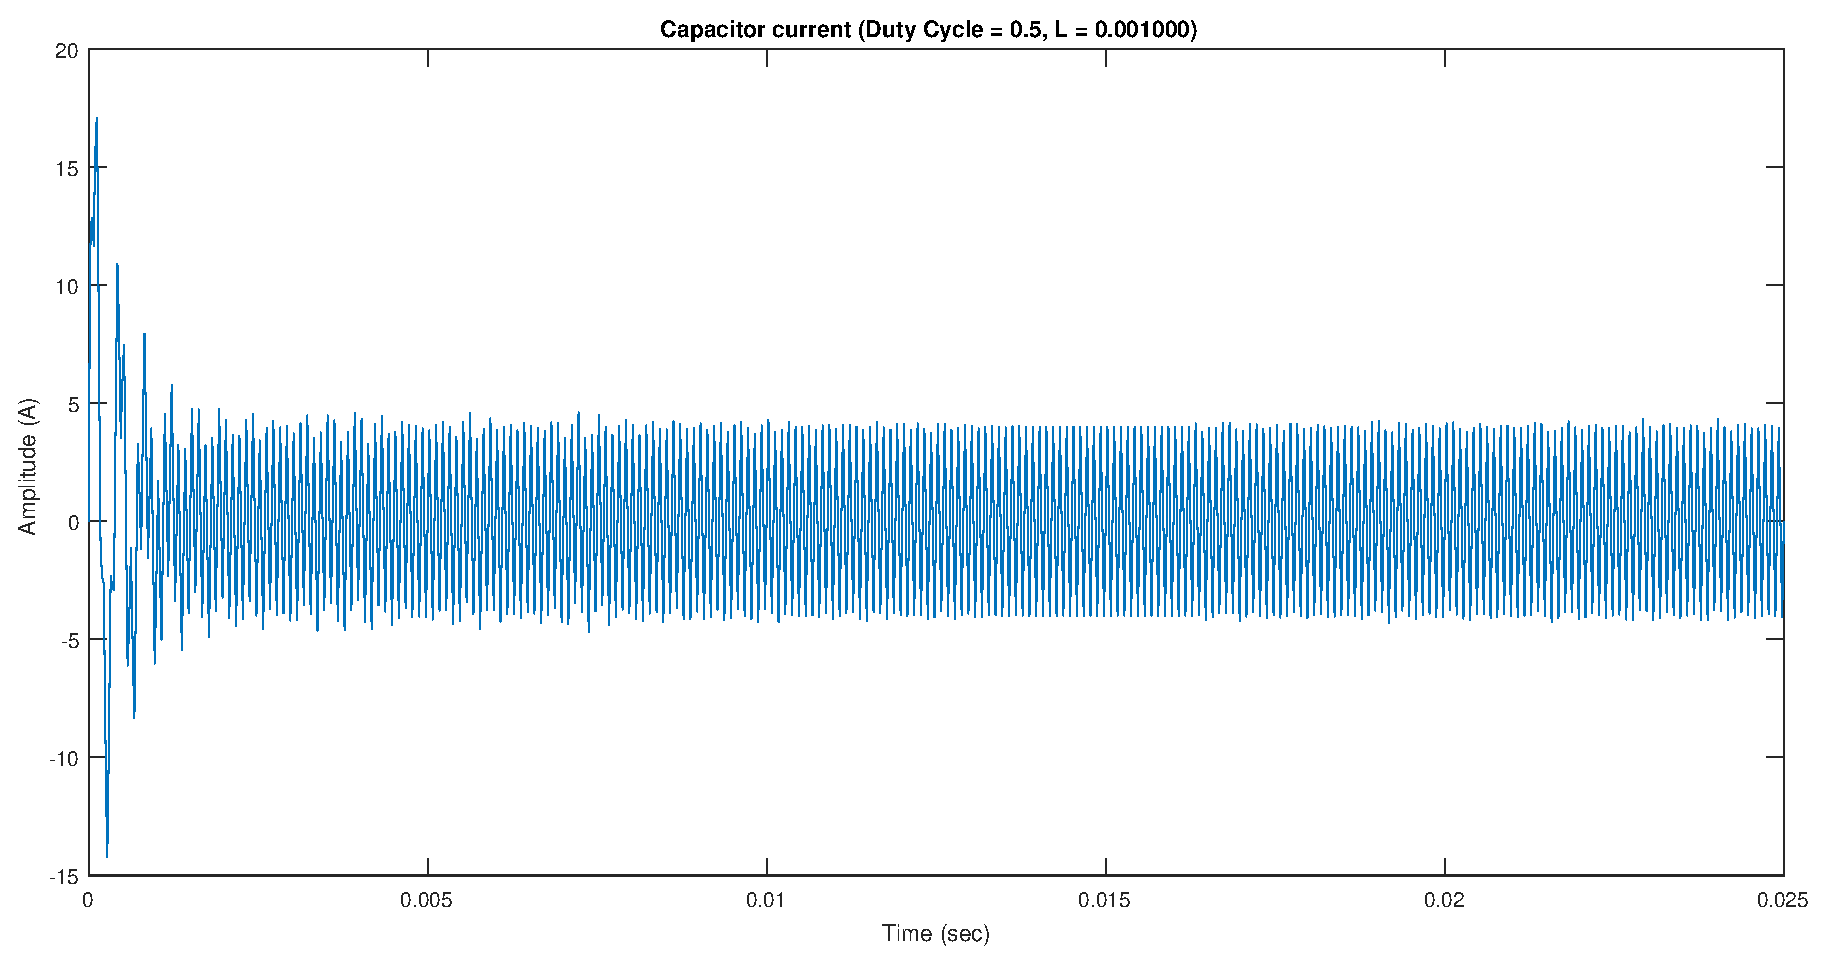
\includegraphics[width=0.8\textwidth]{Images/I_C_05_1}
\end{figure}

\clearpage


\subsubsection{Τάση πυκνωτή}
\subsection{Duty Cycle = 0.5  -  L = 0.01H}
\subsubsection{Ρεύμα πηνίου}
\subsubsection{Ρεύμα πυκνωτή}
\subsubsection{Τάση πυκνωτή}
\subsection{Duty Cycle = 0.8  -  L = 0.001H}
\subsubsection{Ρεύμα πηνίου}
\subsubsection{Ρεύμα πυκνωτή}
\subsubsection{Τάση πυκνωτή}
\subsection{Σύγκριση επίδρασης παραμέτρων}